\documentclass{article}

\usepackage{hyperref}
\usepackage{pgfplots}
\usepgfplotslibrary{fillbetween}


\title{Basics of Economics}
\author{Alvin Lin}
\date{Principles of Microeconomics: August 2016 - December 2016}

\begin{document}

\maketitle

\section{Markets and Efficiency}
How are goods allocated efficiently? How are goods allocated fairly? A
\textbf{normative statement} is an expression of how things ought to be, and a
\textbf{positive statement} is an expression of how things are.

\subsection{Competitive Market}
Trade occurs at the equilibrium price. Every buyer willing to pay that price
or more gets to buy. Every seller willing to trade at that price or less
gets to sell. A competitive market has no external control. Many individuals
acting in their own self interest determines how resources are allocated.

\subsection{Consumer Surplus}
Consumer surplus is the excess of the benefit received from a good over the
amount paid for it.
\[ \mathrm{consumer\ surplus} = \mathrm{marginal\ benefit}-
   \mathrm{the\ price\ paid} \]

\subsubsection{Example}
Suppose I am willing to pay \$5 for the first cheeseburger and \$4 for the
second but I purchase 2 cheeseburgers at \$3 each. My marginal benefit for the
first cheeseburger was \$5 and my marginal benefit for the second was \$4. The
surplus for the first cheeseburger was \$2 and the surplus for the second
cheeseburger was \$1. The consumer surplus obtained is \$3.

\subsection{Benefit, Cost, and Surplus}
The \textit{marginal benefit} is the value to a person of one more good or
service. We can measure this as the maximum price that a person is willing to
pay for one more unit of a good. An individual's demand curve is their marginal
benefit curve. \textbf{For any individual, the consumer surplus from consuming
q units is the area below the individual's demand curve above the price, up to
q}. \par
\textbf{Individual Demand} is the relationship between the price of a good and
the quantity demanded by a particular individual. \par
\textbf{Market Demand} is the relationship between the price of a good and the
quantity demanded by all the buyers in a market, derived by summing all the
individual quantities demanded at each price.

\subsubsection{Example}
\begin{center}
  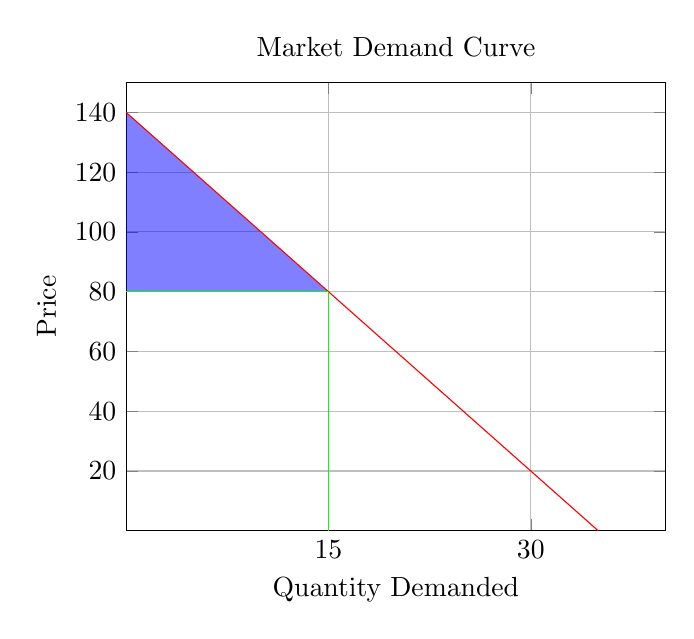
\begin{tikzpicture}
    \begin{axis} [
      title={Market Demand Curve},
      xlabel={Quantity Demanded},
      ylabel={Price},
      xmin=0, xmax=40,
      ymin=0, ymax=150,
      ytick={20,40,60,80,100,120,140},
      xtick={15,30,45},
      grid=both
    ]
    \addplot[name path=path, color=red] coordinates { (0,140) (35,0) };
    \addplot[name path=bound, color=green] coordinates { (0,80) (15,80) };
    \addplot[color=green] coordinates { (15,80)(15,0) };
    \addplot[color=blue, fill=blue, fill opacity=0.5]
      fill between[of=path and bound, soft clip={domain=0:15}];
    \end{axis}
  \end{tikzpicture}
\end{center}
The consumer surplus when price is 80 is the area under the curve above 80.
\[ A = \frac{1}{2}bh = \frac{1}{2}\times15\times60 = 450 \]

\subsection{Producer Surplus}
Producer surplus is the excess of the revenue received from a good over the
amount paid to produce it.
\[ \mathrm{producer\ surplus} = \mathrm{total\ revenue}-\mathrm{total\ cost} \]
Given a price, a supplier will supply the quantity that makes profit (producer
surplus) as large as possible. A producer maximimizes producer surplus (profit)
by choosing the quantity that sets \( P = MC \).

\subsubsection{Market Supply}
Market supply gives tne relationship between price and quantity supplied by the
whole market. It is derived by summing all the \textit{individual quantities
supplied} at each price.

\subsubsection{Market Producer Surplus}
Market producer surplus is the sum of all the individual producer surpluses. It
is calculuated as the area above the market supply function but below the market
price. Given a price, a consumer will demand the quantity that makes her
consumer surplus as large as possible. \par
The quantity supplied is determined by each individual producer supplying the
amount that maximizes her profits. The quantity demanded is determined by each
individual consumer demanding the amount that maximizes his consumer surplus.

\subsubsection{Total Surplus}
The total surplus is the total benefit to society net of all costs.
\[ \mathrm{total\ surplus} = \mathrm{producer\ surplus\ }(PS)+
   \mathrm{consumer\ surplus\ }(CS) \]
Total surplus is maximized in a competitive equilibrium.
\begin{center}
  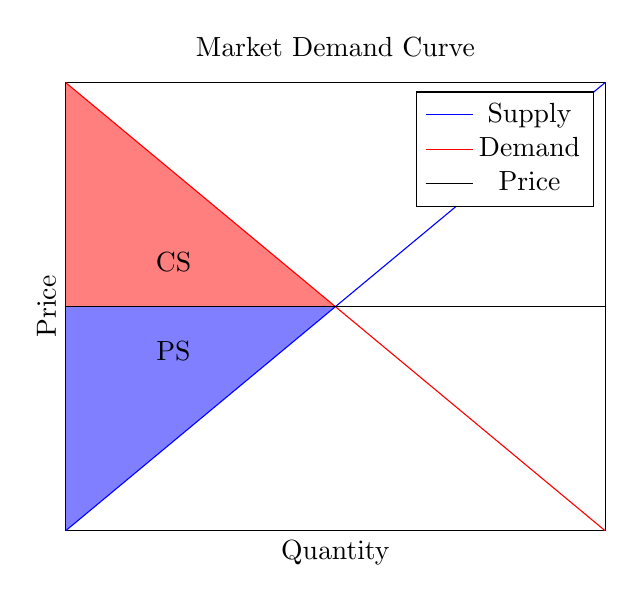
\begin{tikzpicture}
    \begin{axis} [
      title={Market Demand Curve},
      xlabel={Quantity}, ylabel={Price},
      xtick=\empty, ytick=\empty,
      xmin=0, xmax=100, ymin=0, ymax=100
    ]
      \addplot[name path=supply, color=blue] coordinates { (0,0) (100,100) };
      \addlegendentry{Supply};
      \addplot[name path=demand, color=red] coordinates { (0,100) (100,0) };
      \addlegendentry{Demand};
      \addplot[name path=split, color=black] coordinates { (0,50) (100,50) };
      \addlegendentry{Price};
      \addplot[color=blue, fill=blue, fill opacity=0.5]
        fill between [of=split and supply, soft clip={domain=0:50}];
      \addplot[color=red, fill=red, fill opacity=0.5]
        fill between [of=split and demand, soft clip={domain=0:50}];
      \node[draw=none] at (20,60) {CS};
      \node[draw=none] at (20,40) {PS};
    \end{axis}
  \end{tikzpicture}
\end{center}

\subsection{Market Failure}
When there is a fixed price imposed on a good, there can be different
effects on consumers and producers.
\begin{center}
  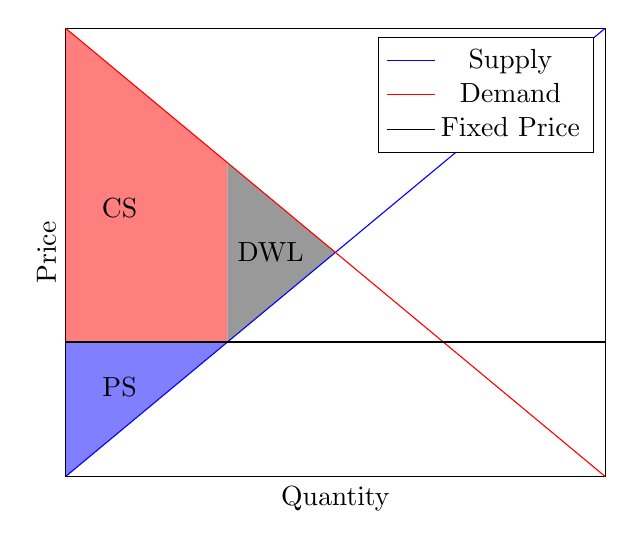
\begin{tikzpicture}
    \begin{axis} [
      xlabel={Quantity}, ylabel={Price},
      xtick=\empty, ytick=\empty,
      xmin=0, xmax=100, ymin=0, ymax=100
    ]
      \addplot[name path=supply, color=blue] coordinates { (0,0) (100,100) };
      \addlegendentry{Supply};
      \addplot[name path=demand, color=red] coordinates { (0,100) (100,0) };
      \addlegendentry{Demand};
      \addplot[name path=split, color=black] coordinates { (0,30) (100,30) };
      \addlegendentry{Fixed Price};
      \addplot[color=blue, fill=blue, fill opacity=0.5]
        fill between [of=split and supply, soft clip={domain=0:30}];
      \addplot[color=red, fill=red, fill opacity=0.5]
        fill between [of=split and demand, soft clip={domain=0:30}];
      \addplot[color=black, fill=black!40]
        fill between [of=supply and demand, soft clip={domain=30:50}];
      \node[draw=none] at (10,60) {CS};
      \node[draw=none] at (10,20) {PS};
      \node[draw=none] at (38,50) {DWL};
    \end{axis}
  \end{tikzpicture}
  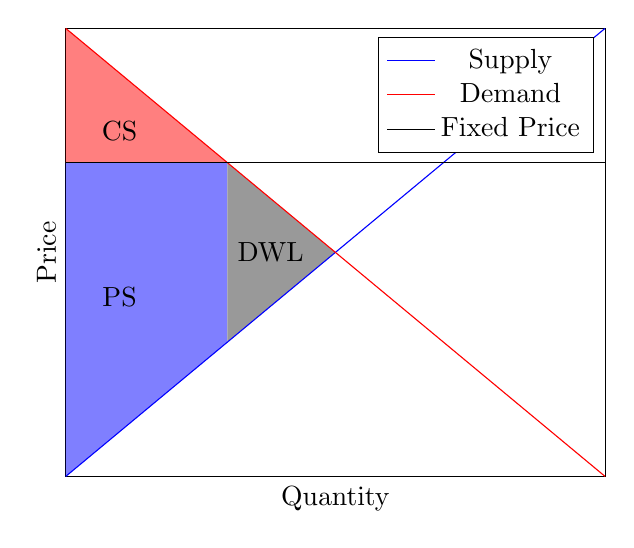
\begin{tikzpicture}
    \begin{axis} [
      xlabel={Quantity}, ylabel={Price},
      xtick=\empty, ytick=\empty,
      xmin=0, xmax=100, ymin=0, ymax=100
    ]
      \addplot[name path=supply, color=blue] coordinates { (0,0) (100,100) };
      \addlegendentry{Supply};
      \addplot[name path=demand, color=red] coordinates { (0,100) (100,0) };
      \addlegendentry{Demand};
      \addplot[name path=split, color=black] coordinates { (0,70) (100,70) };
      \addlegendentry{Fixed Price};
      \addplot[color=blue, fill=blue, fill opacity=0.5]
        fill between [of=split and supply, soft clip={domain=0:30}];
      \addplot[color=red, fill=red, fill opacity=0.5]
        fill between [of=split and demand, soft clip={domain=0:30}];
      \addplot[color=black, fill=black!40]
        fill between [of=supply and demand, soft clip={domain=30:50}];
      \node[draw=none] at (10,77) {CS};
      \node[draw=none] at (10,40) {PS};
      \node[draw=none] at (38,50) {DWL};
    \end{axis}
  \end{tikzpicture}
\end{center}
The triangle of surplus lost is called dead-weight loss (DWL). It represents
the decrease in total surplus resulting from an inefficient level of production.
This is a situation called market failure where a market fails to achieve an
efficient outcome and happens because of overproduction or underproduction. \par
Amount of trade can also affect dead-weight loss. Let \( TS* \) be the optimal
total surplus at the competitive equilibrium quantity \( Q* \). If the quantity
traded is \( \neq Q* \), then \( TS < TS* \).
\begin{center}
  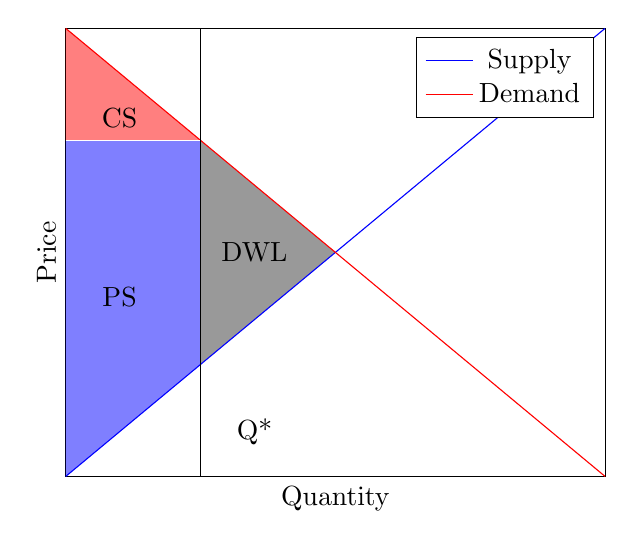
\begin{tikzpicture}
    \begin{axis} [
      xlabel={Quantity}, ylabel={Price},
      xtick=\empty, ytick=\empty,
      xmin=0, xmax=100, ymin=0, ymax=100
    ]
      \addplot[name path=supply, color=blue] coordinates { (0,0) (100,100) };
      \addlegendentry{Supply};
      \addplot[name path=demand, color=red] coordinates { (0,100) (100,0) };
      \addlegendentry{Demand};
      \addplot[name path=split, color=white] coordinates { (0,75) (25,75) };
      \addplot[name path=q, color=black] coordinates { (25,0) (25,100) };
      \addplot[color=blue, fill=blue, fill opacity=0.5]
        fill between [of=split and supply, soft clip={domain=0:25}];
      \addplot[color=red, fill=red, fill opacity=0.5]
        fill between [of=split and demand, soft clip={domain=0:25}];
      \addplot[color=black, fill=black!40]
        fill between [of=supply and demand, soft clip={domain=25:50}];
      \node[draw=none] at (10,80) {CS};
      \node[draw=none] at (10,40) {PS};
      \node[draw=none] at (35,50) {DWL};
      \node[draw=none] at (35,10) {Q*};
    \end{axis}
  \end{tikzpicture}
\end{center}

\subsubsection{Sources of Market Failure}

\paragraph{Price and Quantity Regulation:}
Price regulations such as rent control or minimum wage or quantity regulations
such as quotas can cause market failure.

\paragraph{Taxes and Subsidies:}
Taxes and subsidies can incentivize or deincentivize production of a good.

\paragraph{Externalities:}
An externality is a cost or benefit to someone other than the seller or buyer.
If the externality imposes a cost on an outside party, then there is
overproduction relative to what is socially optimal. If the externality provides
a benefit to an outside party, then there is underproduction relative to what is
socially optimal.

\paragraph{Public Goods and Common Resources:}
A public good is a good with usage that cannot be regulated and that can be
consumed by many persons simultaneously, such as national defense and clean air.
Common resources are resources owned by no particular individual but available
to everyone.

\paragraph{Monopoly:}
A monopoly is a firm that is the sole supplier of a good or service.

\paragraph{High Transaction Costs:}
Transaction costs are the costs required for the market to operate.

\begin{center}
  You can find all my notes at \url{http://omgimanerd.tech/notes}. If you have
  any questions, comments, or concerns, please contact me at
  alvin@omgimanerd.tech
\end{center}

\end{document}
